\documentclass[9pt]{beamer-control}
\usepackage{beamer-control-prac}
\begin{document}
\TOPIC[3]{Frequency Domain}
\CONCEPT[5]{Week 5: Frequency domain modelling}

\begin{frame}
\frametitle{Introduction}
In this practical, we will move onto the compound pendulum system and be introduced to frequency domain methods.

\vfill

This practical will consist of the following parts:
\begin{itemize}
\item Second-order systems
\item Controlling the plant
\item Frequency response
\end{itemize}
\end{frame}

\SUBCONCEPT{Second-order systems}

\begin{frame}{Compound pendulum}

In this practical we will use the compound pendulum system.
Grab the yellow compound pendulum and position the QUBE on its side, such that the pendulum is appropriately affected by gravity.\\

\begin{figure}
	\centering
	\includegraphics[width=6cm]{prac5_pendulum.png}
	\caption{QUBE with compound pendulum attachment.}
\end{figure}

\end{frame}


\begin{frame}{Compound pendulum}
	We begin by deriving a model of the system.
The nonlinear equation of motion for the pendulum is 
\[\tau(t) = (J_m+J_h+J_p) \ddot{\theta}(t) + D_r \dot{\theta}(t) + m_b r_p g \sin \left(\theta (t)\right), \]
where $\tau$ is the torque applied to the joint and $\theta$ is the angular displacement of the pendulum. The constants in this equation are the moments of inertia of the mass, hub, and pendulum $J_m$, $J_h$, and $J_p$, the mass of the bob $m_b$, centre of gravity of the pendulum $r_p$, viscous damping of the pivot $D_r$, and the gravitational acceleration $g$.\\

Using the small angle approximation, applying the Laplace transform, and rearranging the second-order transfer function for the compound pendulum is 
\[ G(s) = \frac{\theta(s)}{\tau (s)} = \frac{1}{(J_m+J_h+J_p)s^2 + D_r s + m_b r_p g } .\]

\end{frame}


\begin{frame}{Compound pendulum}
The parameter values for the QUBE compound pendulum are $R_m=8.4\Omega$, $k_m=0.042$ V/(rad/s), $D_r=2\times 10^{-5}$ N.m.s/rad, $J_m = 4\times 10^{-6}$ kg.m$^2$, $J_h = 0.65 \times 10^{-6}$ kg.m$^2$, $m_b=0.03$ kg, $m_p=0.095$ kg, $r_b = 0.0127$ m, and $r_p = 0.035$ m.
The moment of inertia of a pendulum is given by the parallel axis theorem as $J_p = m_b r_p^2+ \tfrac{1}{2}m_b r_b^2$.

The second-order transfer function may be transformed into a two-dimensional linear state-space model given by the matrices
\[
\mathbf{A}=\begin{bmatrix}
	0 & 1 \\
	-\tfrac{m_br_p g }{J_m+J_h+J_p} & -\left(\tfrac{R_m D_r + k_m^2}{R_m(J_m+J_h+J_p)}\right)
\end{bmatrix},
\mathbf{B} = \begin{bmatrix}
	0 \\ \tfrac{k_m}{R_m(J_m+J_h+J_p)}
\end{bmatrix}, 
\mathbf{C} = \begin{bmatrix}
	1 & 0
\end{bmatrix},
\mathbf{D} = \begin{bmatrix}
	0
\end{bmatrix}
\]  
where 
\[\mathbf{x} = \begin{bmatrix}
	\theta_m \\ \dot{\theta}_m
\end{bmatrix}
\quad , \quad \mathbf{y} = \theta_m \quad  \text{and} \quad u=v_m.\]
\end{frame}



\SUBCONCEPT{Controlling the plant}

\begin{frame}{Pole placement}

Given the transfer function model of the compound pendulum, one method of control is to design state feedback such that the resulting poles of the closed loop system provide a desired response

For a general second-order system, the pair of complex poles are given by  
\[s=\omega_n (-\zeta_n \pm j \sqrt{1-\zeta_n^2})\]

\begin{figure}
	\centering
	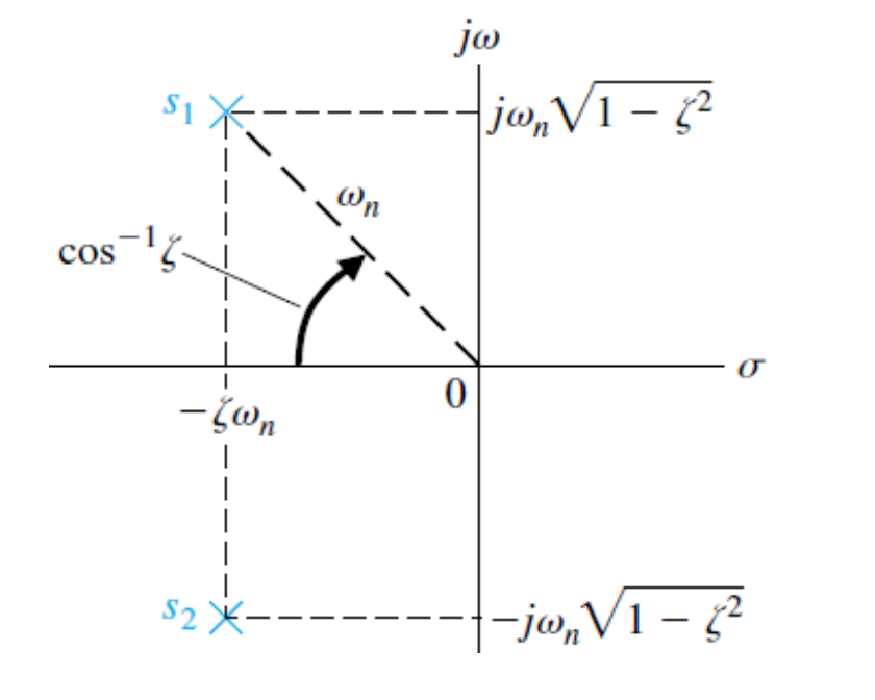
\includegraphics[width=5cm]{prac5_poles}
	\caption{Plot of a pair of complex poles.}
\end{figure}


\end{frame}



\begin{frame}{Pole placement}

\begin{enumerate}
	\item Calculate the position of the desired poles given that we require a damping ratio of $\zeta_n=\tfrac{1}{2\sqrt{2}}$ with a natural frequency of $\omega_n=10$ rad/s
	\item Calculate the $A$ and $B$ matrices in Matlab and use the command K=place(A,B,p) to determine the required gains 
	\item Implement this controller in Simulink by multiplying the appropriate states with the corresponding gain values (you will have to estimate the angular velocity $\dot{\theta}$ using a low-pass filter and a derivative block)
	\item Run the system with no input and apply an impulse to the system by tapping the bottom of the pendulum (or model an impulse in Simulink using a Step block)
	\item Calculate the theoretical damped natural frequency $\omega_d=\omega_n\sqrt{1-\zeta^2}$, does the impulse response match what you would expect? Why or why not?
	\item Try again with $\omega_n=2$ rad/s and compare
\end{enumerate}

Why is pole placement not a robust control strategy?

\end{frame}


\begin{frame}{Pole placement}

\begin{figure}
	\centering
	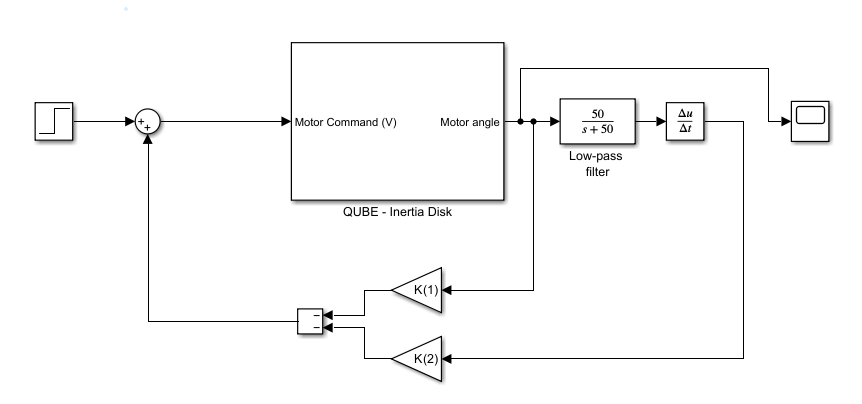
\includegraphics[width=\linewidth]{prac5_poleplacement}
	\caption{Simulink setup for pole placement.}
\end{figure}

\end{frame}


\begin{frame}{Command tracking}
\begin{itemize}
	\item With only proportional and derivative gain we cannot in general achieve perfect command tracking and must include feedback of the integral of the error
	\item Now adding a step input of $\tfrac{\pi}{4}$ to your Simulink model, evaluate the step response of your pole placement controller
	\item You should find that despite being able to successfully change the location of the poles of our system, our step response has non-zero steady state error and therefore falls short at accurately tracking our input
	\item We therefore need to include integral feedback which we will do by using PID control
\end{itemize}

\end{frame}

\begin{frame}{PID Control}
Similar to last week, we may characterise the open loop output response of the pendulum system as an FOTD model.

\begin{enumerate}
	\item Characterise the step response of the open-loop compound pendulum as a FOTD model by finding the parameters $a$, $T$, and $\tau$
	\item Using these FOTD parameters, select a PID tuning law and determine the corresponding PID gains
	\item Run the system in close loop with a step input of $\tfrac{\pi}{4}$
	
\end{enumerate}

After implementing the tuned PID gains, manually tune your controller to improve your step response.

\end{frame}



\SUBCONCEPT{Frequency response}

\begin{frame}{Response to a sinusoid input}
With a controller implemented and optimised, we often would like to understand how well our controller can follow a given input. One way to assess this that gives us more information than just looking at the system's response to a step input is to input a periodic signal and analyse the phase and magnitude of the output.

\begin{enumerate}
	\item Replace the Step block in Simulink with a Signal Generator block, change to a sinusoid signal, and set the frequency to 1 Hz and the amplitude to $\tfrac{\pi}{4}$
	\item Run the Simulink and assess how well the controller follows this signal by plotting both the input and output signals on one Scope
\end{enumerate}

\end{frame}



\begin{frame}{Next week}
	This week we moved onto the compound pendulum system, derived its model, and controlled it with several different strategies. We also analysed the performance of the controller at following a sinusoidal input.
	
	Next week we will experimentally analyse the frequency response of the compound pendulum plant to a range of frequencies to better assess and understand the performance of a system.
\end{frame}



\end{document}
